\section{Introduction}
\label{section:introduction}

The realistic representation of the flow around wind turbines and larger wind parks can have a valuable impact on many fields. In engineering, it enables the optimization of turbine design and control to minimize structural loads and maximize power outputs. Economic assessments of the cost of wind energy production rely on a thorough understanding of how much energy a wind park will produce, and how often load-induced maintenance and replacements are necessary. Policy makers and planners are interested in the local environmental effects from acoustics to microclimates to regulate the placement of wind parks effectively.\\

To gain understanding of the aerodynamic effects of wind turbines, simulation tools are invaluable as they allow to study numerous conditions and arrangements without the need of complex experiments. However, the simulation of fluid dynamics at the scale of wind turbines or whole wind parks comes with a considerable trade-off. Detailed, high-fidelity simulations may capture the physics of the problem accurately, but are computationally very expensive. An alternative can be found in low-fidelity engineering models which model the physical phenomena in a simplified way to represent the most important aspects of the problem at hand. A popular engineering model for the fluid-structure interaction of wind turbines is the Actuator Line Method (ALM) \cite{Churchfield:2017}. The turbine tower and blades are represented as slender beams or lines, reducing the number of computational nodes. Nevertheless, it allows the detailed study of blade deformations and wake effects. 
A widely-used tool implementing the Actuator Line Method is the wind turbine simulation software OpenFAST\footnote{\url{https://openfast.readthedocs.io/en/main/}}. Coupling OpenFAST with a high-fidelity CFD solver allows to accurately solve the wind field at moderate computational cost. 
The CFD program computes a detailed large-scale flow field and exchanges the local flow velocity with OpenFAST (see Fig. \ref{fig:openfast:coupling}). OpenFAST computes the turbine dynamics and sends back forces and deflections which are imposed on the flow field. The challenge in this setup lies in implementing the data exchange and mapping while ensuring numerical robustness of the simulation.\\

One solution to this problem is the open-source tool preCICE. preCICE is a coupling library for multi-physics simulations and allows to couple different programs to perform a partitioned simulation. It takes care of the communication and data mapping between the tools and implements different coupling schemes. To connect a program to preCICE, an additional piece of software called adapter is necessary. Once a simulation tool is connected to preCICE, it can be coupled to any other program in the preCICE environment, reducing the time-to-solution. The main idea of this work is therefore to develop a preCICE-OpenFAST adapter to couple OpenFAST to CFD simulation tools via preCICE.\\

To provide context, chapter \ref{section:review} provides a literature review on the existing couplings between OpenFAST and several CFD solvers. The software packages used as well as the concept of the newly developed module are then described in chapter \ref{section:software}. Chapter \ref{section:cases} outlines two example cases on which the software is applied, followed by a description of the development challenges the software still faces to reach maturity in chapter \ref{section:challenges}. The final chapter \ref{section:conclusion} concludes on the current capabilities and future possibilities of this approach.

\begin{comment}
The big picture
\\
 \begin{itemize}
 	\item Understanding the flow in wind parks can have a valuable impact on many fields
 	\begin{itemize}
 		\item Engineering: Optimize turbine design and control to minimize load while maximizing power output
 		\item Economics: Assess the economic viability
 		\item Environment and Policy: Impact on the local environment and how to regulate it
 	\end{itemize}
 	\item While the detailed, high-fidelity simulation of turbines is computationally very expensive, low-fidelity engineering models present an alternative
 	\item Model the physical phenomena in a simplified way to represent the most important aspects for the problem at hand
 	\item A popular engineering model for wind turbines is the Actuator Line Method
 	\item Turbine tower and blades are represented as slender beams
 	\item Allows the detailed study of wake effects and blade deformations
 	\item Open-source tool OpenFAST implements such models
 	\item Coupling OpenFAST with a high-fidelity LES CFD solver would allow to accurately solve the wind field at moderate computational cost \ref{fig:openfast:coupling}
 	\item preCICE is a multi-physics coupling library to couple different solvers
 	\item Coupled tools include OpenFOAM, an open-source CFD solver used in industry and academia
 	\item To couple a tool via preCICE, an additional piece of software called adapter is necessary
 	\item Idea: Write a preCICE-OpenFAST adapter to couple OpenFAST to CFD solvers via preCICE
 	\\
 \end{itemize}
\end{comment}

\begin{figure*}[h]
	\centering
	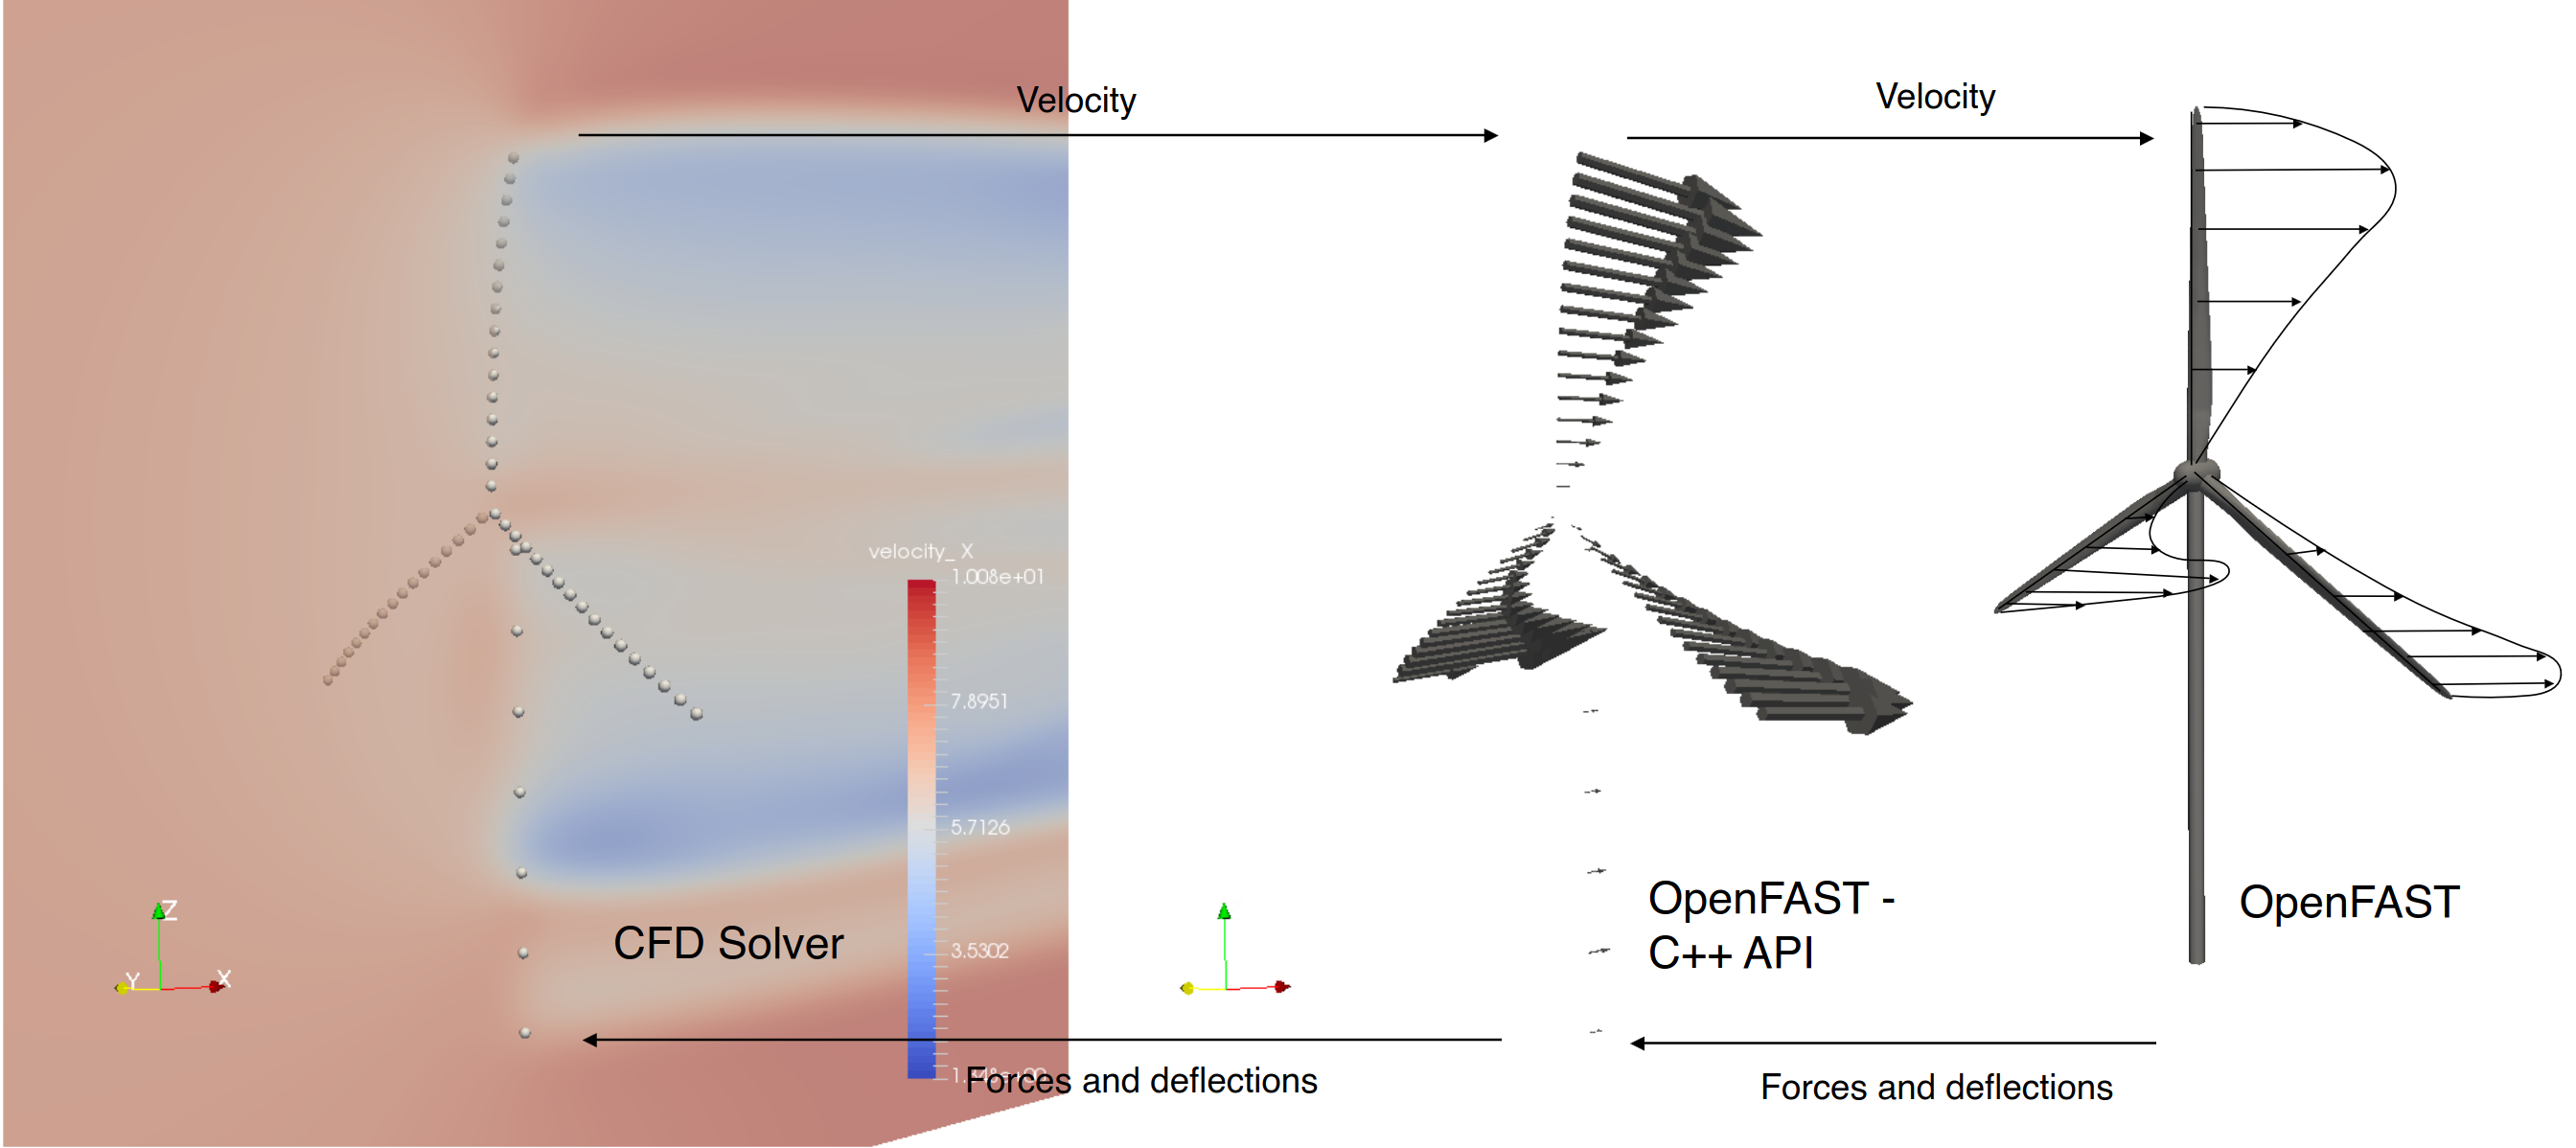
\includegraphics[width=0.9\textwidth]{images/openfast-coupling-scheme.png}
	\caption{Coupling of OpenFAST to a CFD program. The fluid solver computes the flow dynamics and sends velocity data to OpenFAST. OpenFAST simulates the turbine dynamics and sends back forces and deflections, which are imposed on the flow field. Source: OpenFAST documentation\protect\footnotemark}
	\label{fig:openfast:coupling}
\end{figure*}

\footnotetext{{\url{https://ganesh-openfast.readthedocs.io/en/latest/_images/actuatorLine_illustrationViz.pdf}(visited on 07.11.2023)}}

